\documentclass[10pt,tgadventor, onlymath]{beamer}

\usepackage{graphicx,amsmath,amssymb,tikz,psfrag,neuralnetwork, stackengine,array, multirow}

\input defs.tex
\graphicspath{ {./figures/} }

%% formatting

\mode<presentation>
{
\usetheme{default}
\usecolortheme{seahorse}
}
\setbeamertemplate{navigation symbols}{}
\usecolortheme[rgb={0.03,0.28,0.59}]{structure}
\setbeamertemplate{itemize subitem}{--}
\setbeamertemplate{frametitle} {
	\begin{center}
	  {\large\bf \insertframetitle}
	\end{center}
}

\newcommand\footlineon{
  \setbeamertemplate{footline} {
    \begin{beamercolorbox}[ht=2.5ex,dp=1.125ex,leftskip=.8cm,rightskip=.6cm]{structure}
      \footnotesize \insertsection
      \hfill
      {\insertframenumber}
    \end{beamercolorbox}
    \vskip 0.45cm
  }
}
\footlineon

\AtBeginSection[] 
{ 
	\begin{frame}<beamer> 
		\tableofcontents[currentsection,currentsubsection] 
	\end{frame} 
} 


\usetikzlibrary{shapes,arrows}
\usetikzlibrary{positioning}
\tikzstyle{block} = [rectangle, draw, fill=blue!20, 
    text width=5em, text centered, rounded corners, minimum height=4em]
\tikzstyle{line} = [draw, -latex']



%% begin presentation

\title{\large \bfseries Power Allocation in Heterogeneous Networks for Base Stations with Multiple Antennas}

\author{Peter Hartig\\[3ex]
}

\date{\today}

\begin{document}

\frame{
\thispagestyle{empty}
\titlepage
}

\section{System Description}
\begin{frame}
\frametitle{The Heterogeneous Network}
TODO get image of network
\end{frame}

\begin{frame}
\frametitle{Players of the Game}
Femto Cell Base Stations (FC-BSs) are characterized by the following:
\begin{itemize}
\item 
	Each FC-BS  $f \in \{1 ... F\}$ has $T_f$ antennas with which to transmit to $K_f$  users with  $T_f \geq K_f$.
\\
\item 
	FC-BSs  can beamform using the precoding 	
	matrix $\mathbf{U}_{\mathrm{f}} \in \mathbb{C}_{T_f \times K_f}$ such that the transmitted 		
	signal is $\mathbf{s}_{\mathrm{f}
	}= \mathbf{U_{\mathrm{f}}}\mathbf{x_{\mathrm{f}}}$ with $E[\|\mathbf{x}_{\mathrm{f}}\|_2^2 = 1]$.
\\
\item 
	FC-BS $f$ has power constraint $trace(\mathbf{U}_f^H\mathbf{U}_f) \leq P^{Total}_{f} $.
\\
\item
	 FC-BSs are assumed to be spaced such that FC-BS $f$ causes no interference to the users of FC-BS $j \in \{1 ... F\}\backslash f$
\item 
	FC-BSs has utility function $U_f()$ based upon the quality of service 		
	provided to its users. TODO (Discuss Reasonable functions)
\\
\item 
	FC-BS $f$ knows the downlink channel ($\mathbf{H_\mathrm{f}}$) from its transmission antennas to all served users.
\\
\item
	The interference tolerance of macro cell users cannot be exceeded 
\end{itemize}

\end{frame}


\begin{frame}
\frametitle{The Heterogeneous Network Game}
\begin{columns}

\begin{column}{0.5\linewidth}
Image of HetNet
\end{column}
\begin{column}{0.5\linewidth}
\begin{table}
    \setlength{\extrarowheight}{2pt}
    \begin{tabular}{cc|c|c|}
      & \multicolumn{1}{c}{} & \multicolumn{2}{c}{Player $2$}\\
      & \multicolumn{1}{c}{} & \multicolumn{1}{c}{$A$}  & \multicolumn{1}{c}{$B$} \\\cline{3-4}
      \multirow{2}*{Player $1$}  & $A$ & $(8,8)$ & $(2,15)$ \\\cline{3-4}
      & $B$ & $(15,2)$ & $(3,3)$ \\\cline{3-4}
    \end{tabular}
  \end{table}
\end{column}
\end{columns}

\end{frame}

\begin{frame}
\frametitle{Objectives}
\begin{enumerate}
\item Find a Nash Equilibrium between all players.
\begin{itemize}
\item Preferably, one which is unique and close a social optimum.
\end{itemize}
\item Achieve a Nash Equilibrium in a distributed solution.
\begin{itemize}
\item Minimize communication overhead in system to reach Nash Equilibrium.
\end{itemize}
\end{enumerate}

\begin{center}
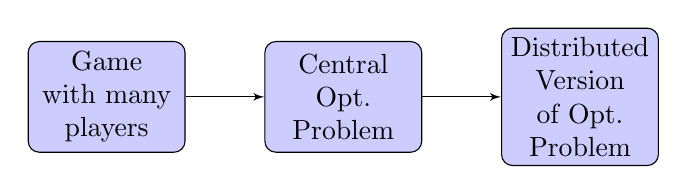
\begin{tikzpicture}{center}
\node [block] (game) {Game with many players};
\node [block, right = of game] (central) {Central Opt. Problem};
\node [block, right = of central] (distributed) {Distributed Version of Opt. Problem};

\path[line] (game) -- (central);
\path[line] (central) -- (distributed);

\end{tikzpicture}
\end{center}
\end{frame}


\end{document}
